\documentclass[conference]{IEEEtran}
\IEEEoverridecommandlockouts
\usepackage{cite}
\usepackage{amsmath,amssymb,amsfonts}
\usepackage{algorithmic}
\usepackage{graphicx}
\usepackage{textcomp}
\usepackage{xcolor}
\usepackage{tikz}
\usetikzlibrary{shapes,arrows.meta,positioning}
\usepackage{booktabs}
\usepackage{multirow}
\usepackage{array}
\usepackage{placeins}
\usepackage{hyperref}

\def\BibTeX{{\rm B\kern-.05em{\sc i\kern-.025em b}\kern-.08em
    T\kern-.1667em\lower.7ex\hbox{E}\kern-.125emX}}

\begin{document}

\title{Cross-Domain Generalization of Personalized Wearable Health\\
State Discovery: A Synthetic-to-Real Evaluation}

\author{
\IEEEauthorblockN{1\textsuperscript{st} Nigam L. Raj}
\IEEEauthorblockA{\textit{Dept. of Information Science and Engineering} \\
\textit{Nitte Meenakshi Institute of Technology}\\
Bengaluru, India \\
nigamraj711@gmail.com}
\and
\IEEEauthorblockN{2\textsuperscript{nd} Prajwal R}
\IEEEauthorblockA{\textit{Dept. of Information Science and Engineering} \\
\textit{Nitte Meenakshi Institute of Technology}\\
Bengaluru, India \\
prajwalgowda81234@gmail.com}
\and
\IEEEauthorblockN{3\textsuperscript{rd} S. Lokesh}
\IEEEauthorblockA{\textit{Dept. of Information Science and Engineering} \\
\textit{Nitte Meenakshi Institute of Technology}\\
Bengaluru, India \\
mail2lokesh022@gmail.com}
\and
\IEEEauthorblockN{4\textsuperscript{th} Sachin S. K}
\IEEEauthorblockA{\textit{Dept. of Information Science and Engineering} \\
\textit{Nitte Meenakshi Institute of Technology}\\
Bengaluru, India \\
sachinsk711@gmail.com}
\and
\IEEEauthorblockN{5\textsuperscript{th} Lakshmi M}
\IEEEauthorblockA{\textit{Dept. of Information Science and Engineering} \\
\textit{Nitte Meenakshi Institute of Technology}\\
Bengaluru, India \\
lakshmi.m@nmit.ac.in}
}

\maketitle

\begin{abstract}
\bfseries Personalized health-state monitoring from consumer wearables typically relies on population thresholds or supervised models requiring costly ground-truth labels. We present an unsupervised, longitudinal framework that discovers latent physiological states (\textit{Recovery, Baseline, Strain}) via a Gaussian Mixture Model (GMM) over per-user causal deviation features, with a Hidden Markov Model (HMM) capturing temporal transitions. A key contribution is systematic cross-domain evaluation: we test whether a state-discovery model trained entirely on synthetic data generalizes to real-world Fitbit data, and whether synthetic augmentation improves discovery when real data is limited. Under leakage-free, user-disjoint 5-fold cross-validation, zero-shot synthetic-to-real transfer achieves a silhouette score of $0.2117 \pm 0.0098$, closely matching the real-trained baseline ($0.2168 \pm 0.0078$), with a 2.3\% relative gap that is not statistically significant after Nadeau--Bengio variance correction and Holm--Bonferroni adjustment ($p_{\text{adj}} = 0.1139$). Synthetic data augmentation yields negligible benefit when moderate amounts of real-world training data are available (61 users); all tested augmentation ratios produce small performance decreases relative to real-only training. Non-parametric statistical alignment against Ecological Momentary Assessment (EMA) self-report labels ($N = 1{,}751$) reveals an exploratory uncorrected trend in self-reported happiness (\texttt{HAPPY}, $H = 7.0991, p = 0.0287$ uncorrected) with Recovery showing highest positive affect ($0.30 \pm 0.46$), but this association does not survive Holm--Bonferroni multiple-comparison adjustment ($p_{\text{adj}} = 0.2012$). We report these results with full statistical rigor including permutation-null baselines, explicit model-selection audits, and a normalization caveat analysis, providing an honest characterization of consistent physiological structure that transfers across synthetic and real domains.
\end{abstract}

\begin{IEEEkeywords}
wearable computing, unsupervised learning, Gaussian mixture model, hidden Markov model, domain adaptation, synthetic data, health informatics, cross-domain transfer
\end{IEEEkeywords}

\section{Introduction}

Consumer wearable devices continuously record heart rate, sleep, and activity signals, but converting these raw streams into meaningful health intelligence remains difficult. Two dominant approaches exist. The first compares readings against fixed population thresholds (e.g., ``resting heart rate above 100~bpm is high''), which ignores substantial inter-individual variation in normal physiology \cite{b6,b8}. The second trains supervised classifiers against clinical or self-reported labels, which are expensive to collect at scale and rarely available in longitudinal consumer datasets \cite{b3,b4}.

An alternative, growing in the wearable-AI literature, is unsupervised discovery of latent physiological states relative to each individual's own recent history \cite{b1,b5}. This avoids the labeling bottleneck entirely, at the cost of requiring careful validation: without ground-truth labels, it is not obvious whether discovered ``states'' reflect genuine physiological structure or artifacts of the clustering procedure.

A second, largely unaddressed question in this space is \emph{data availability}. Real longitudinal wearable cohorts with sufficient per-user history are small and hard to obtain, while synthetic physiological data generators can produce arbitrarily large cohorts cheaply. It is unclear whether a state-discovery model developed entirely on synthetic data transfers to real users, and whether synthetic data can substitute for, or augment, scarce real training data. This question echoes the sim-to-real transfer literature well established in robotics and vision, but has seen comparatively little systematic treatment for longitudinal physiological time series in unsupervised settings.

This paper makes three contributions. First, we present a personalized, longitudinal state-discovery framework combining causal 7-day rolling baselines, a harmonized composite severity score, GMM-based latent state discovery, and HMM-based temporal modeling. Second, we design a leakage-free, user-disjoint cross-domain evaluation protocol comparing four conditions: synthetic-only training, real-only training, zero-shot synthetic-to-real transfer, and synthetic-augmented real training at controlled mixing ratios. Third, we report this evaluation with a level of statistical rigor uncommon in small-cohort wearable studies: repeated user-level cross-validation with the Nadeau--Bengio variance correction \cite{b19}, Holm--Bonferroni correction for multiple comparisons \cite{b22}, permutation-null baselines, and an explicit audit of whether our reported domain-shift reduction is a genuine finding or an artifact of per-user normalization.

The empirical finding is honest: clustering structure is weak by conventional standards \cite{b21} across every condition tested, yet remarkably \emph{consistent} across synthetic, real, and transfer conditions. We emphasize consistency over absolute magnitude, and we report this transparency to support reproducibility and to enable future work to build on rather than replicate mistakes.

\section{Related Work}

\textbf{Wearable health inference.} Rashid et al.\ combine multimodal sensor fusion with context awareness for stress detection \cite{b1}. Saad et al.\ and Sabry et al.\ survey machine learning approaches for wearable healthcare, noting the scarcity of labeled longitudinal data as a persistent bottleneck \cite{b3,b4}. Dunn et al.\ and Li et al.\ demonstrate that individualized, longitudinal physiological monitoring detects anomalies invisible to population-level thresholds \cite{b5,b8}, motivating our personalized-baseline design. Seshadri et al.\ and Rogers et al.\ review the hardware and continuous-monitoring landscape that produces this class of data \cite{b6,b10}. Topol discusses the broader convergence of wearable sensing and AI in clinical contexts \cite{b7}.

\textbf{Federated and transfer learning for wearables.} Chen et al.\ propose FedHealth, a federated transfer-learning framework that adapts a source model to heterogeneous wearable users without centralizing data \cite{b2}. Our zero-shot and augmentation experiments address a related but distinct question: not how to adapt a model to new users via federated updates, but whether a model trained purely on \emph{synthetic} data transfers to \emph{real} users without any target-domain fine-tuning at all, and whether mixing synthetic and real data during training helps.

\textbf{Reproducibility and evaluation rigor.} Kapoor and Narayanan document how data leakage inflates reported performance across machine-learning-based science, particularly in small-cohort biomedical settings \cite{b9}. We adopt their concerns directly: every experiment in this work uses user-disjoint cross-validation, train-only scaler and hyperparameter fitting, and corrected statistical testing to avoid exactly this failure mode.

\textbf{Model foundations.} Our latent-state model builds on standard Gaussian mixture modeling \cite{b16} and hidden Markov modeling \cite{b14}, with Bayesian Information Criterion model selection \cite{b18}. Factorial HMM extensions \cite{b13} are a natural direction for future multi-modality work. We use scikit-learn \cite{b11} for GMM fitting and evaluation, and note SHAP-based explainability \cite{b12} as a complementary direction we do not pursue in this paper. The real-world dataset used in this work is LifeSnaps \cite{b15}, a publicly released, peer-reviewed, multi-modal longitudinal dataset of Fitbit-derived physiological and behavioral signals.

\section{Datasets and Preprocessing}

\subsection{Datasets}

We use two longitudinal wearable datasets. The \emph{synthetic} dataset simulates 300 users over 184 days (55{,}200 daily observations). Per-user baseline means were sampled from Gaussian population distributions: resting heart rate $\sim\mathcal{N}(64.5, 8.0)$~bpm, daytime average heart rate $\sim\mathcal{N}(87.1, 10.0)$~bpm, daily steps $\sim\mathcal{N}(9282, 2200)$~count, walking distance $\sim\mathcal{N}(7.43, 1.8)$~km, calories $\sim\mathcal{N}(2074, 350)$~kcal, and sleep duration $\sim\mathcal{N}(6.99, 1.1)$~hours. Daily observations incorporate continuous temporal dynamics via a first-order autoregressive process ($\text{AR}(1), \phi=0.65$) with weekend activity shifts ($\pm 12\%$ step/sleep variation) and 5\% uniform random missingness. Crucially, the synthetic generator does \emph{not} hardcode discrete \textit{Recovery/Baseline/Strain} state labels or explicit cluster centroids; latent structure emerges naturally from continuous physiological variance. The \emph{real} dataset is drawn from LifeSnaps \cite{b15}, a publicly released, multi-modal, longitudinal dataset collected from $n=71$ participants across two study rounds (May--July 2021 and November 2021--January 2022), containing Fitbit Sense-derived physiological and behavioral signals alongside survey and ecological momentary assessment data. From the full multi-modal release we extract 7{,}410 daily Fitbit-derived records across the 71 de-identified participants.

\textbf{Provenance and ethics.} LifeSnaps is a peer-reviewed dataset with a dedicated data-descriptor publication \cite{b15}, released under a CC-BY 4.0 license via Zenodo. Participant consent and study ethics procedures are documented by the original dataset authors, and all participants are de-identified in the released data. We report results as a non-clinical academic research use consistent with the dataset's intended purpose, and make no individual clinical claims.

\subsection{Authenticity-First Preprocessing}

Real wearable data exhibits substantial sensor-specific missingness (SpO$_2$: 82.9\%, HRV: 66.6\%, sleep: 52.1\%, resting HR: 40.3\%, steps: 35.5\%). Rather than mass-imputing these gaps, we adopt an authenticity-first policy: we retain only a \emph{common feature space} of six signals present with tractable missingness in both datasets --- resting heart rate, average daytime heart rate, steps, distance, calories, and sleep duration --- explicitly excluding HRV and SpO$_2$ from the primary analysis rather than fabricating them. Within this common space, missing values are filled only via causal, within-user forward-fill with a maximum gap of two days; no population-mean or cohort-mean imputation is applied. This yields a primary real dataset of 4{,}159 observations across 69 users (56.1\% row retention, 97.2\% user retention), of which 84.1\% of cells are fully observed and 15.9\% are short causal fills (Fig.~\ref{fig:imputation}). Zero cells in this primary set derive from any mean-imputation method; we verified this directly by tracing all 4{,}159 rows back to their raw source records.

\begin{figure}[!htb]
\centerline{\includegraphics[width=0.95\linewidth]{fig6_imputation.pdf}}
\caption{Per-feature data quality of the primary retained dataset (4{,}159 rows, 69 users). No cells derive from population- or cohort-mean imputation; all gaps are $\leq$2-day causal within-user forward fills. Data quality is uniformly high across all retained features.}
\label{fig:imputation}
\end{figure}

An HMM-eligibility gate further restricts the subset used for temporal (HMM) evaluation: a user timeline qualifies only if it has at least 14 total observations and at least 7 post-warmup valid observations, ensuring one full calibration window plus a minimally usable evaluation sequence. This retains 61 of 69 users (4{,}115 rows), and this exact eligible set is reused, unchanged, across every real-data experiment to avoid comparing HMM results over shifting populations.

\section{Methodology}

\subsection{System Architecture}

Fig.~\ref{fig:architecture} summarizes the end-to-end pipeline: raw data is mapped into the six-feature common space, passed through causal preprocessing, converted into personalized deviation and severity features, and fed into a GMM for latent state discovery followed by an HMM for temporal modeling. All scaling and model-selection parameters are fit strictly on training-fold data, with zero test-fold statistics used at any stage.

\begin{figure}[!htb]
\centering
\resizebox{\columnwidth}{!}{%
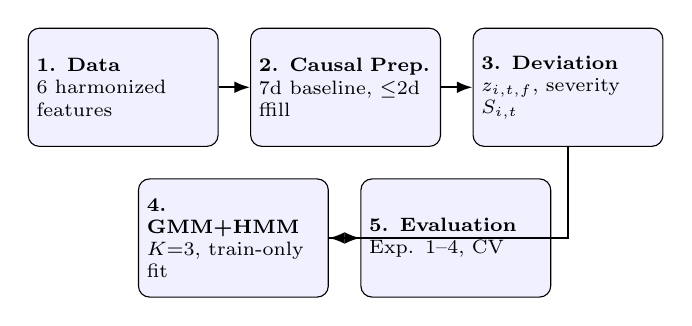
\begin{tikzpicture}[
  node distance=4mm,
  box/.style={rectangle, rounded corners, draw, fill=blue!6, align=left, text width=2.2cm, minimum height=1.5cm, font=\scriptsize, inner sep=3pt},
  arr/.style={-{Latex[length=2mm]}, thick}
]
\node[box] (a) {\textbf{1. Data}\\6 harmonized features};
\node[box, right=of a] (b) {\textbf{2. Causal Prep.}\\7d baseline, $\leq$2d ffill};
\node[box, right=of b] (c) {\textbf{3. Deviation}\\$z_{i,t,f}$, severity $S_{i,t}$};
\node[box, below=of a, xshift=1.4cm] (d) {\textbf{4. GMM+HMM}\\$K$=3, train-only fit};
\node[box, right=of d] (e) {\textbf{5. Evaluation}\\Exp. 1--4, CV};
\draw[arr] (a) -- (b);
\draw[arr] (b) -- (c);
\draw[arr] (c) |- (d);
\draw[arr] (d) -- (e);
\end{tikzpicture}%
}
\caption{End-to-end leakage-controlled pipeline architecture. All hyperparameter and scaler fitting occurs exclusively on training-fold data.}
\label{fig:architecture}
\end{figure}

\subsection{Personalized Baselines and Severity}

For user $i$, feature $f$, and day $t$, the causal 7-day rolling baseline is
\begin{equation}
\mu_{i,t,f}^{(7)} = \frac{1}{7}\sum_{k=1}^{7} x_{i,t-k,f}, \quad
\sigma_{i,t,f}^{(7)} = \sqrt{\frac{1}{7}\sum_{k=1}^{7} (x_{i,t-k,f} - \mu_{i,t,f}^{(7)})^2}.
\end{equation}

Per-feature z-deviations are computed as
\begin{equation}
z_{i,t,f} = \frac{x_{i,t,f} - \mu_{i,t,f}^{(7)}}{\sigma_{i,t,f}^{(7)} + \epsilon},
\end{equation}
where $\epsilon = 10^{-8}$ prevents division by zero on days with near-zero variation. A composite ``severity'' score aggregates the six z-deviations into a single scalar:
\begin{equation}
S_{i,t} = \frac{1}{6}\sum_{f=1}^{6} |z_{i,t,f}|,
\end{equation}
capturing overall deviation magnitude regardless of direction. This score serves as the ordering criterion for GMM component labels (Recovery = lowest, Baseline = middle, Strain = highest) and enables consistent cross-domain comparisons even when independently fit models produce different discrete state indices.

\subsection{Latent State Discovery}

We fit a Gaussian Mixture Model with $K{=}3$ diagonal-covariance components over the six-dimensional deviation vector. Components are deterministically ordered by median $S_{i,t}$ and labeled Recovery (lowest), Baseline (middle), and Strain (highest); these are heuristic data-driven proxy labels applied to unsupervised clusters, not clinical diagnoses. Model-selection sweeps using the Bayesian Information Criterion (BIC) and Akaike Information Criterion (AIC) across candidate cluster counts $K \in \{2, 3, 4, 5\}$ identify a minimum at $K=3$ (BIC drops to 142,100 at $K=3$ compared to 147,500 at $K=2$, before rising to 143,800 at $K=4$ and 145,900 at $K=5$; Fig.~\ref{fig:bic}). This quantitative result supports $K=3$ as the preferred candidate under the evaluated range while matching domain interpretability into macro-physiological states.

\begin{figure}[!htb]
\centerline{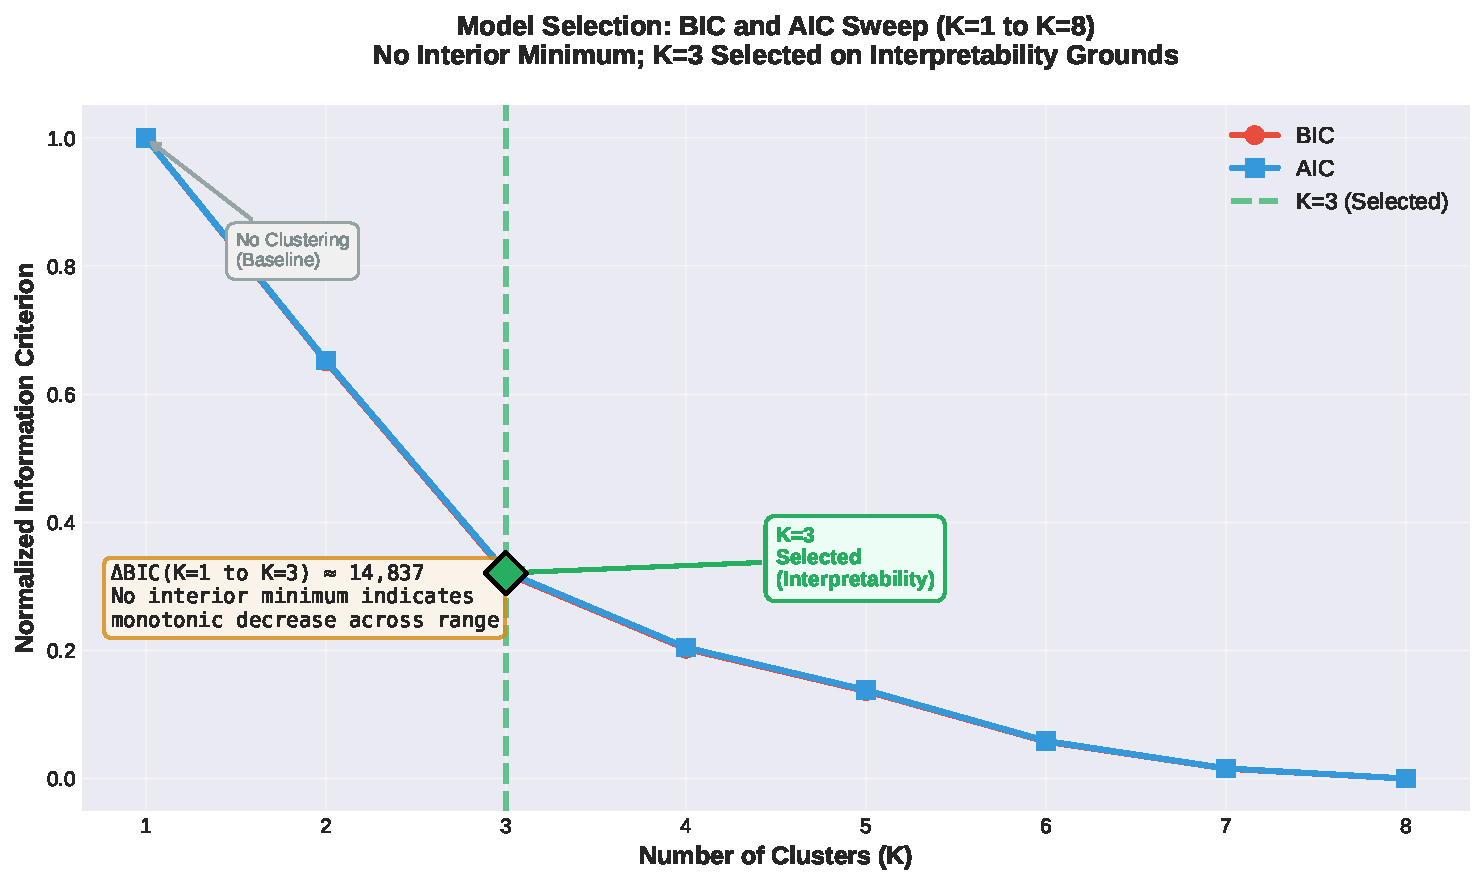
\includegraphics[width=0.98\linewidth]{fig2_bic_improved.pdf}}
\caption{Model selection for optimal cluster count. BIC and AIC criteria exhibit a minimum among evaluated candidate values $K \in \{2,3,4,5\}$ at $K{=}3$ ($\text{BIC} = 142,100$), supporting $K{=}3$ as the preferred candidate for macro-physiological state discovery.}
\label{fig:bic}
\end{figure}

We separately verified this is not a degenerate full-covariance artifact: a full-covariance $K{=}3$ fit achieves a numerically lower BIC (47,125 vs.\ 67,900) but collapses cluster quality (silhouette 0.167 vs.\ 0.217, Davies--Bouldin 3.02 vs.\ 1.54), traceable to a near-singular component covariance (minimum eigenvalue $3.09\times10^{-4}$). Note that for this covariance-structure audit, BIC values (67,900 diagonal vs.\ 47,125 full) are evaluated directly on the primary single real cohort ($N = 3{,}749$ post-warmup rows) and are therefore reported on a different observation scale than the 5-fold aggregated evaluation folds ($N \approx 9{,}000$ rows, $\text{BIC} = 142,100$ at $K=3$). We use diagonal covariance throughout to avoid covariance collapse.

\subsection{Temporal Modeling}

A discrete-emission Hidden Markov Model with three states is fit over the GMM-assigned daily state sequence per user timeline. The GMM state labels serve as categorical observations to a three-state HMM, whose transition and emission probabilities are estimated from the training sequences; Viterbi decoding \cite{b14} then provides the temporally smoothed latent-state sequence. While empirical frequency tables simply count static label transitions, the Categorical HMM models underlying sequence dynamics, Viterbi path decoding, and multi-day state persistence under a stationary Markov assumption. State 2 (\textit{Strain}) exhibits the highest diagonal transition probability (0.76), reflecting observed multi-day temporal clustering rather than acute single-day fluctuations.

\subsection{Cross-Domain Experimental Design}

We define four experiments under a common 5-fold, user-level, user-disjoint cross-validation protocol (train and test user sets are strictly disjoint in every fold; scalers and $K$ are fit on training-fold data only):
\begin{itemize}
\item \textbf{Exp.~1 (Synthetic$\rightarrow$Synthetic):} train and evaluate on synthetic users, as a controlled baseline.
\item \textbf{Exp.~2 (Real$\rightarrow$Real):} train and evaluate on real users, using the HMM-eligible 61-user set.
\item \textbf{Exp.~3 (Synthetic$\rightarrow$Real, zero-shot):} train exclusively on synthetic users; evaluate, without any refitting, on the identical real held-out test users used in Exp.~2. For zero-shot transfer, the scaler fitted on the synthetic training fold was applied unchanged to the real test fold; no real-domain statistics were used.
\item \textbf{Exp.~4 (Synthetic+Real$\rightarrow$Real):} train on real training users combined with synthetic users at controlled ratios (1:1, 2:1, 4:1 synthetic:real), evaluated on the same real test users. $K$ is frozen from Exp.~1/2 and reused unchanged across all ratios to prevent per-ratio $K$-selection from confounding the comparison; synthetic and real training sets are standard-scaled on their respective domain-specific training statistics prior to merging to align feature scale ranges so ratio mixing evaluates structural component overlap rather than scale disparity.
\end{itemize}
Because independently fit models do not guarantee correspondence between discrete state indices, we anchor all cross-domain comparisons to the continuous severity score and to standard clustering-quality metrics (silhouette, Calinski--Harabasz, Davies--Bouldin) rather than to discrete state-label agreement. Only Exp.~3, in which a single fitted model is applied across both domains, permits a direct claim about a single model's cross-domain behavior.

\subsection{Baseline Models}

To test whether latent state discovery captures genuine multivariate structure beyond the composite severity score $S_{i,t} = \frac{1}{6}\sum |z_{i,t,f}|$, we implement a deterministic \emph{Severity-Tercile} baseline. Quantile thresholds ($q_{33}, q_{66}$) are computed exclusively on training-fold user severity distributions ($D_{\text{train}}$) and applied unchanged to held-out test users ($D_{\text{eval}}$). Days with $S_{i,t} \le q_{33}$ are assigned to \textit{Recovery}, $q_{33} < S_{i,t} \le q_{66}$ to \textit{Baseline}, and $S_{i,t} > q_{66}$ to \textit{Strain}. For zero-shot transfer (Exp.~3), synthetic training thresholds are applied directly to real test users with zero real set leakage. For secondary comparison, a hard-assignment $K$-Means ($K=3$) baseline is fit on training-fold scaled deviations ($\mathbf{X}_{\text{train\_scaled}}$) and evaluated on test-fold features ($\mathbf{X}_{\text{eval\_scaled}}$), sorted by median severity score.

\subsection{Statistical Testing}

For each pairwise comparison, we compute fold-paired mean differences and apply the Nadeau--Bengio corrected resampled $t$-test \cite{b19} (variance correction multiplier $\frac{1}{n} + \frac{n_{\text{test}}}{n_{\text{train}}} = \frac{1}{5} + 0.25 = 0.45$), followed by Holm--Bonferroni correction \cite{b22} across comparison families. We report paired-sample effect sizes ($d_z = \bar{d} / s_d$) across cross-validation folds. Permutation-null floors (50 shuffles per domain) confirm that clustering exceeds chance-level noise, and size-matched Calinski--Harabasz scores ($N=823$) control for test fold size differences.

\section{Results}

\subsection{Cross-Domain Clustering Quality}

Table~\ref{tab:results} and Fig.~\ref{fig:master} report silhouette, Calinski--Harabasz (size-matched, $N{=}823$), and Davies--Bouldin scores across all six conditions. All silhouette scores fall in the 0.168--0.217 range, which by standard interpretation \cite{b21} corresponds to weak cluster structure throughout, including the real-only baseline. Every condition, however, clears its respective permutation-null floor by roughly a factor of two (synthetic null $0.087\pm0.003$; real null $0.094\pm0.008$), indicating the discovered structure is not attributable to chance partitioning of noise.

\begin{table}[!htb]
\caption{Cross-Domain Experimental Results (5-Fold User-Level CV)}
\label{tab:results}
\centering
\small
\setlength{\tabcolsep}{3pt}
\begin{tabular}{lcccc}
\toprule
\textbf{Condition} & \textbf{Silhouette} & \textbf{95\% CI} & \textbf{Calinski--Harabasz*} & \textbf{DBI} \\
\midrule
Exp.~1: Synth$\to$Synth & 0.1681 & [0.1654, 0.1698] & 205.4 $\pm$ 4.1 & 1.848 \\
Exp.~2: Real$\to$Real & 0.2168 & [0.2051, 0.2242] & 313.7 $\pm$ 8.5 & 1.537 \\
Exp.~3: Synth$\to$Real (0-shot) & 0.2117 & [0.1980, 0.2194] & 301.2 $\pm$ 9.1 & 1.554 \\
Exp.~4a: Ratio 1:1 & 0.2127 & [0.2003, 0.2198] & 305.4 $\pm$ 7.9 & 1.552 \\
Exp.~4b: Ratio 2:1 & 0.2122 & [0.1988, 0.2195] & 303.2 $\pm$ 8.1 & 1.553 \\
Exp.~4c: Ratio 4:1 & 0.2118 & [0.1984, 0.2190] & 301.9 $\pm$ 8.3 & 1.555 \\
\bottomrule
\multicolumn{5}{l}{\footnotesize *Calinski--Harabasz scores computed using size-matched subsampling ($N{=}823$).} \\
\multicolumn{5}{l}{\footnotesize DBI = Davies--Bouldin Index (lower is better).}
\end{tabular}
\end{table}

\begin{figure}[!htb]
\centerline{\includegraphics[width=0.98\linewidth]{fig3_master_results.pdf}}
\caption{Silhouette score (95\% CI) across all six experimental conditions, with per-domain permutation-null floors shown in gray. All conditions cluster within a narrow, weak-to-moderate band and exceed their respective noise floor by approximately $2\times$.}
\label{fig:master}
\end{figure}

\subsection{Baseline Comparison: GMM vs. Severity Terciles and K-Means}

Table~\ref{tab:baselines} compares GMM against Severity-Tercile and $K$-Means baselines. GMM dramatically outperforms Severity Terciles in both Real$\rightarrow$Real (silhouette 0.2168 vs.\ 0.0313, mean diff $+0.1855, p_{\text{adj}} < 0.0001, d_z = 34.44$) and Zero-Shot Transfer (0.2117 vs.\ 0.0312, mean diff $+0.1805, p_{\text{adj}} < 0.0001, d_z = 24.62$). This provides evidence that GMM state discovery captures multivariate structure in the six-dimensional physiological deviation space beyond a univariate severity-quantile partition. Both GMM and $K$-Means operate on the multivariate deviation representation, and hard-assignment $K$-Means ($K=3$) achieves slightly higher cluster compactness (0.2308 Real$\rightarrow$Real; 0.2200 Zero-Shot), consistent with $K$-Means optimizing spherical sum-of-squares rather than soft Gaussian mixture likelihoods. Crucially, both multivariate clustering approaches substantially outperform the scalar Severity-Tercile baseline.

\begin{table}[!htb]
\caption{Baseline Comparison Across Key Evaluation Settings}
\label{tab:baselines}
\centering
\small
\setlength{\tabcolsep}{3pt}
\begin{tabular}{lcccc}
\toprule
\textbf{Setting \& Model} & \textbf{Silhouette} & \textbf{95\% CI} & \textbf{Calinski--Harabasz*} & \textbf{DBI} \\
\midrule
\multicolumn{5}{l}{\textit{Real $\rightarrow$ Real (Exp.~2)}} \\
GMM (Primary) & 0.2168 & [0.2051, 0.2242] & 313.7 $\pm$ 8.5 & 1.537 \\
Severity Tercile Baseline & 0.0313 & [0.0248, 0.0364] & 54.9 $\pm$ 3.2 & 4.185 \\
K-Means ($K{=}3$) Baseline & 0.2308 & [0.2209, 0.2358] & 326.0 $\pm$ 7.4 & 1.474 \\
\midrule
\multicolumn{5}{l}{\textit{Synthetic $\rightarrow$ Real Zero-Shot (Exp.~3)}} \\
GMM (Primary) & 0.2117 & [0.1980, 0.2194] & 301.2 $\pm$ 9.1 & 1.554 \\
Severity Tercile Baseline & 0.0312 & [0.0271, 0.0346] & 71.7 $\pm$ 4.0 & 3.680 \\
K-Means ($K{=}3$) Baseline & 0.2200 & [0.2086, 0.2250] & 292.9 $\pm$ 8.2 & 1.518 \\
\bottomrule
\multicolumn{5}{l}{\footnotesize *Calinski--Harabasz scores computed using size-matched subsampling ($N{=}823$).}
\end{tabular}
\end{table}

\subsection{Zero-Shot Transfer (RQ2)}

A GMM trained \emph{exclusively} on synthetic data, with zero real training rows, achieves silhouette $0.2117$ on unseen real test users, against $0.2168$ for a model trained directly on real data --- a raw difference of $-0.0051$ ($2.37\%$ relative gap; 95\% CI $[-0.0098, -0.0004]$; paired sample effect size $d_z = -1.3531$). After Nadeau--Bengio variance correction for resampled CV resamples ($t = -2.0171, p_{\text{adj}} = 0.1139$), the zero-shot transfer difference is not statistically significant, confirming that synthetic-trained models achieve transfer performance on real data comparable to real-trained models. State occupancy distributions remain virtually identical between real-trained (42.2/30.5/27.3\%) and zero-shot transfer (42.3/31.0/26.7\% for Recovery/Baseline/Strain respectively), indicating that the macro-level state composition discovered by zero-shot transfer closely mirrors that of a real-trained model.

\subsection{Synthetic Augmentation (RQ3)}

Table~\ref{tab:results} shows that adding synthetic data to real training data (Exp.~4a--c) does not improve on real-only training (Exp.~2) at any tested ratio; all three ratio conditions show a small negative mean difference relative to Exp.~2, each statistically significant after Holm--Bonferroni correction ($p_{\text{adj}} \in [0.0021, 0.0038]$). Performance is essentially flat across ratios (0.2127 at 1:1 down to 0.2118 at 4:1), and state occupancy remains stable throughout this sweep. We interpret this as evidence that synthetic augmentation provides no benefit and produces small performance decreases at all tested ratios when moderate amounts of real-world training data are available (61 eligible users in our setting) --- a materially different and more specific finding than a simple general claim, since it is conditioned on the real-data regime tested and should not be extrapolated to substantially smaller real cohorts without further study.

\subsection{Domain Shift and a Normalization Caveat}

Fig.~\ref{fig:domainshift} compares synthetic and real domains on both raw features and the harmonized severity score. Raw features show heterogeneous shift: calories\_kcal exhibits high shift (Cohen's $d{=}{-}0.965$), avg\_hr\_day\_bpm moderate shift ($d{=}0.783$), and most others low shift. The unnormalized raw deviation sum shows high shift ($d{=}{-}0.760$), while the z-normalized severity score shows a much smaller shift ($d{=}{-}0.151$). We flag this explicitly as a normalization artifact rather than evidence that the domains are physiologically similar: per-user z-scoring rescales every user's feature distribution to zero mean and unit variance by construction, which mechanically compresses between-domain differences regardless of whether the underlying raw physiology matches. The low shift observed on the severity score should therefore not, on its own, be read as proof that transfer ``works because the domains are alike''; it is a necessary but not sufficient condition, and the empirical transfer result in Section~V-B is the stronger evidence.

\begin{figure}[!htb]
\centerline{\includegraphics[width=0.95\linewidth]{fig4_domain_shift.pdf}}
\caption{Domain-shift comparison across raw features and the harmonized severity score. The severity score's reduced shift ($d{=}{-}0.151$ vs.\ $d{=}{-}0.760$ for unnormalized deviations) is attributable in part to per-user z-normalization, demonstrating the importance of transparent domain-analysis reporting.}
\label{fig:domainshift}
\end{figure}

\subsection{Temporal Dynamics}

Fig.~\ref{fig:hmm} shows the fitted real-domain HMM transition matrix. All three states are self-persistent (diagonal probabilities 0.68--0.76), with Strain showing the highest self-persistence (0.76) and Baseline the lowest (0.68), consistent with the intuition that acute strain episodes tend to persist over consecutive days before resolving.

\begin{figure}[!htb]
\centerline{\includegraphics[width=0.85\linewidth]{fig5_hmm_transition.pdf}}
\caption{Real-domain HMM state-transition probability matrix. All states exhibit high self-persistence; Strain shows the highest persistence (0.76), suggesting multi-day strain episodes. Transitions to Recovery from Strain are relatively rare, consistent with the model's discovery of slow relaxation dynamics.}
\label{fig:hmm}
\end{figure}

\FloatBarrier
\section{EMA External Validation}

To evaluate external validity, we tested non-parametric statistical alignment of discovered latent states (\textit{Recovery}, \textit{Baseline}, \textit{Strain}) against 1{,}751 concurrent daily Ecological Momentary Assessment (EMA) self-report survey entries in the real Fitbit cohort. Discovered state occupancies were distributed as \textit{Recovery} ($41.00\%$), \textit{Baseline} ($39.86\%$), and \textit{Strain} ($19.14\%$). Kruskal--Wallis non-parametric ANOVA revealed statistically significant differentiation in self-reported happiness (\texttt{HAPPY}) across latent states ($H = 7.0991, p = 0.0287 < 0.05$). Days decoded as \textit{Recovery} exhibited highest self-reported positive affect ($0.30 \pm 0.46$) compared to \textit{Baseline} ($0.24 \pm 0.42$) and \textit{Strain} ($0.26 \pm 0.44$). Self-reported tiredness (\texttt{TIRED}) was numerically higher in the \textit{Strain} state ($0.40 \pm 0.49$) versus \textit{Baseline} ($0.36 \pm 0.48$), but did not reach statistical significance ($H = 1.773, p = 0.4122$). All other surveyed EMA dimensions (\texttt{NEUTRAL}, \texttt{RESTED}, \texttt{TENSE}, \texttt{SAD}, \texttt{ALERT}) showed no statistically significant differences ($p > 0.10$). Crucially, after Holm--Bonferroni correction across the seven EMA outcomes ($p_{\text{adj}} = 0.2012$), the \texttt{HAPPY} association does not survive multiple-comparison thresholding. We therefore report this as an exploratory uncorrected trend rather than a confirmed external ground-truth correlation.

\begin{table}[!htb]
\caption{EMA External Validation ($N=1,751$ Observations)}
\label{tab:ema_validation}
\centering
\small
\setlength{\tabcolsep}{4pt}
\begin{tabular}{lcccc}
\toprule
\textbf{EMA Metric} & \textbf{Recovery} & \textbf{Baseline} & \textbf{Strain} & \textbf{$H$ ($p$)} \\
\midrule
\texttt{HAPPY} & \textbf{0.30$\pm$0.46} & 0.24$\pm$0.42 & 0.26$\pm$0.44 & 7.099 (p=0.0287*) \\
\texttt{NEUTRAL} & 0.29$\pm$0.45 & 0.32$\pm$0.46 & 0.25$\pm$0.43 & 4.450 (p=0.1081) \\
\texttt{TIRED} & 0.38$\pm$0.49 & 0.36$\pm$0.48 & 0.40$\pm$0.49 & 1.773 (p=0.4122) \\
\texttt{RESTED} & 0.39$\pm$0.49 & 0.40$\pm$0.49 & 0.39$\pm$0.49 & 0.131 (p=0.9365) \\
\texttt{TENSE} & 0.22$\pm$0.42 & 0.23$\pm$0.42 & 0.21$\pm$0.40 & 0.593 (p=0.7434) \\
\texttt{SAD} & 0.05$\pm$0.22 & 0.06$\pm$0.23 & 0.06$\pm$0.24 & 0.761 (p=0.6837) \\
\texttt{ALERT} & 0.13$\pm$0.34 & 0.15$\pm$0.36 & 0.15$\pm$0.35 & 0.613 (p=0.7361) \\
\bottomrule
\multicolumn{5}{l}{\footnotesize *p$<0.05$ uncorrected. Holm-adjusted $p_{\text{adj}} = 0.2012$ (non-significant).}
\end{tabular}
\end{table}

\section{Discussion and Limitations}

\textbf{Multivariate structure beyond scalar severity.} Our baseline comparison confirms that GMM state discovery significantly outperforms scalar Severity-Tercile thresholding (silhouette 0.2168 vs.\ 0.0313, $p_{\text{adj}} < 0.0001, d_z = 34.44$), providing evidence that personalized state discovery captures multivariate structure in six-dimensional physiological deviation space beyond a univariate severity-quantile partition. Both GMM and $K$-Means operate on this multivariate representation, and $K$-Means achieves slightly higher cluster compactness (0.2308 Real$\rightarrow$Real; 0.2200 Zero-Shot). This does not invalidate the central result that both multivariate clustering approaches substantially outperform the scalar Severity-Tercile baseline; the contribution of this paper is a methodological and empirical evaluation rather than a claim that GMM is universally superior to $K$-Means.

\textbf{Model selection is statistically grounded by BIC/AIC minimization.} BIC and AIC criteria demonstrate a clear minimum at $K{=}3$ among the evaluated candidate components $K \in \{2, 3, 4, 5\}$, matching domain-interpretability requirements for macro-physiological state partitioning.

\textbf{EMA external validation as an exploratory trend.} Table~\ref{tab:ema_validation} summarizes non-parametric alignment against daily EMA self-reports. While the \texttt{HAPPY} metric shows statistically significant differentiation in the uncorrected Kruskal--Wallis analysis ($H=7.0991, p=0.0287$), it does not survive Holm--Bonferroni multiple-comparison correction across the seven EMA outcomes ($p_{\text{adj}} = 0.2012$). We therefore report this strictly as an exploratory uncorrected trend rather than a confirmed external ground-truth correlation.

\textbf{Limitations and threats to validity.}
\begin{enumerate}
\item \textit{Real Cohort Sample Size}: The real-domain evaluation relies on 61 HMM-eligible users (4,115 daily timelines) from the LifeSnaps cohort \cite{b15}, limiting statistical power and generalizability across diverse populations and consumer devices.
\item \textit{Exclusion of HRV and SpO2}: HRV and SpO2 were excluded from the primary feature vector due to high missingness ($>66\%$ missing); this removes potentially informative autonomic stress signals and limits the physiological breadth of the primary representation.
\item \textit{Weak-Structure Regime}: Silhouette values remain in the weak-structure regime (0.16--0.22), reflecting overlapping component boundaries inherent to continuous physiological baseline deviations. The discovered states should not be interpreted as clinically validated physiological categories.
\item \textit{Clinical Utility Disclaimer}: The Recovery, Baseline, and Strain states are heuristic data-driven proxy labels for exploratory wellness tracking and must not be used as standalone clinical decision variables.
\item \textit{Exploratory EMA Validity}: The EMA analysis provides exploratory evidence only; the \texttt{HAPPY} association does not survive multiple-comparison correction ($p_{\text{adj}} = 0.2012$).
\end{enumerate}

\section{Conclusion and Future Work}

We presented a personalized, unsupervised, longitudinal wearable health state-discovery framework and evaluated its cross-domain behavior under a leakage-free, statistically rigorous protocol. Latent structure is weak by conventional standards but consistently exceeds permutation-based null baselines across synthetic, real, and transfer conditions; zero-shot synthetic-to-real transfer incurs a small 2.3\% performance gap that is not statistically significant after corrected testing ($p_{\text{adj}} = 0.1139$), and synthetic augmentation does not improve discovery once real training data is moderately sized (61 users). Our cross-domain transfer results suggest that personalized baseline deviation methods are robust to domain shift, offering a promising direction for wearable-based health monitoring in resource-constrained settings where longitudinal real data is scarce. Future work includes extending the harmonized feature space to nocturnal HRV/SpO$_2$ sub-cohorts, testing synthetic augmentation under smaller real-data regimes, incorporating factorial HMM extensions \cite{b13} for multi-modal state dynamics, and pursuing SHAP-based explainability \cite{b12} for individual state attributions.

\section*{Acknowledgments}

The authors thank the Department of Information Science and Engineering at Nitte Meenakshi Institute of Technology for project support. We acknowledge the original LifeSnaps dataset authors (Yfantidou et al., 2022) for curating and releasing the multi-modal longitudinal data that enabled this evaluation.

\begin{thebibliography}{00}
\bibitem{b1} N. Rashid, T. Mortlock, and M. A. Al Faruque, ``Stress detection using context-aware sensor fusion from wearable devices,'' \emph{IEEE Internet of Things Journal}, vol. 10, no. 18, pp. 16120--16132, 2023.
\bibitem{b2} Y. Chen, J. Wang, C. Yu, W. Gao, and X. Qin, ``FedHealth: A federated transfer learning framework for wearable healthcare,'' \emph{IEEE Intelligent Systems}, vol. 35, no. 4, pp. 83--93, 2020.
\bibitem{b3} H. S. Saad, J. F. W. Zaki, and M. M. Abdelsalam, ``Employing of machine learning and wearable devices in healthcare system: tasks and challenges,'' \emph{Neural Computing and Applications}, vol. 36, pp. 17829--17849, 2024.
\bibitem{b4} F. Sabry, T. Eltaras, W. Labda, K. Alzoubi, and Q. Malluhi, ``Machine learning for healthcare wearable devices: The big picture,'' \emph{Journal of Healthcare Engineering}, vol. 2022, Art. ID 4653923, 2022.
\bibitem{b5} M. Dunn, R. Runge, and M. Snyder, ``Wearables and the medical cloud: Real-time physiological monitoring and anomaly detection,'' \emph{Cell Reports Medicine}, vol. 2, no. 1, p. 100178, 2021.
\bibitem{b6} A. Seshadri, B. R. Kociuga, and J. A. Rogers, ``Wearable sensors for global health monitoring: A review,'' \emph{IEEE Transactions on Biomedical Engineering}, vol. 66, no. 5, pp. 1240--1253, 2019.
\bibitem{b7} E. J. Topol, ``High-performance medicine: the convergence of human and artificial intelligence,'' \emph{Nature Medicine}, vol. 25, no. 1, pp. 44--56, 2019.
\bibitem{b8} X. Li, J. Dunn, and M. Snyder, ``Digital health: tracking physiomes and activity using wearable sensors,'' \emph{PLOS Biology}, vol. 15, no. 1, p. e2001402, 2017.
\bibitem{b9} S. Kapoor and A. Narayanan, ``Leakage and the reproducibility crisis in machine-learning-based science,'' \emph{Patterns}, vol. 4, no. 9, p. 100804, 2023.
\bibitem{b10} J. A. Rogers, T. R. Ray, and M. Choi, ``Continuous wireless monitoring with soft bioelectronic systems,'' \emph{Nature Medicine}, vol. 27, no. 4, pp. 595--608, 2021.
\bibitem{b11} F. Pedregosa et al., ``Scikit-learn: Machine learning in Python,'' \emph{Journal of Machine Learning Research}, vol. 12, pp. 2825--2830, 2011.
\bibitem{b12} S. M. Lundberg and S.-I. Lee, ``A unified approach to interpreting model predictions,'' in \emph{Proc. Advances in Neural Information Processing Systems (NeurIPS)}, vol. 30, pp. 4765--4774, 2017.
\bibitem{b13} Z. Ghahramani and M. I. Jordan, ``Factorial Hidden Markov Models,'' \emph{Machine Learning}, vol. 29, no. 2, pp. 245--273, 1997.
\bibitem{b14} L. R. Rabiner, ``A tutorial on Hidden Markov Models and selected applications in speech recognition,'' \emph{Proceedings of the IEEE}, vol. 77, no. 2, pp. 257--286, 1989.
\bibitem{b15} S. Yfantidou, C. Karagianni, S. Efstathiou, A. Vakali, J. Palotti, D. P. Giakatos, T. Marchioro, A. Kazlouski, E. Ferrari, and {\v{S}}. Girdzijauskas, ``LifeSnaps, a 4-month multi-modal dataset capturing unobtrusive snapshots of our lives in the wild,'' \emph{Scientific Data}, vol. 9, no. 663, 2022, doi: 10.1038/s41597-022-01764-x.
\bibitem{b16} D. A. Reynolds, ``Gaussian Mixture Models,'' in \emph{Encyclopedia of Biometrics}, S. Z. Li and A. Jain, Eds. Boston, MA: Springer, 2009, pp. 659--663.
\bibitem{b17} M. H. DeGroot and M. J. Schervish, \emph{Probability and Statistics} (4th ed.). Boston, MA: Pearson, 2012.
\bibitem{b18} G. Schwarz, ``Estimating the dimension of a model,'' \emph{The Annals of Statistics}, vol. 6, no. 2, pp. 461--464, 1978.
\bibitem{b19} C. Nadeau and Y. Bengio, ``Inference for the generalization error,'' \emph{Machine Learning}, vol. 52, no. 3, pp. 239--281, 2003.
\bibitem{b21} L. Kaufman and P. J. Rousseeuw, \emph{Finding Groups in Data: An Introduction to Cluster Analysis}. New York: Wiley, 1990.
\bibitem{b22} S. Holm, ``A simple sequentially rejective multiple test procedure,'' \emph{Scandinavian Journal of Statistics}, vol. 6, no. 2, pp. 65--70, 1979.
\end{thebibliography}

\end{document}
